\documentclass[11pt,a4paper]{article}
\usepackage[T1]{fontenc}
\usepackage[utf8]{inputenc}
\usepackage{lmodern}
\usepackage[margin=27mm]{geometry}
\usepackage{amsmath,amssymb,amsthm,mathtools}
\usepackage{booktabs,microtype}
\usepackage[numbers,sort&compress]{natbib}
\usepackage{xcolor}
\usepackage{tikz}
\usepackage[colorlinks=true,linkcolor=blue!45!black,citecolor=blue!45!black,urlcolor=blue!45!black]{hyperref}
\hypersetup{pdftitle={Coherent information in uniformly noisy graph states is not ordered by subsystem size},pdfauthor={Xiaojian Zeng}}
\newcommand{\F}{\mathbb F_2}
\newcommand{\IA}{\mathcal I_A}
\newcommand{\IB}{\mathcal I_B}
\newcommand{\Tr}{\operatorname{Tr}}
\newcommand{\rank}{\operatorname{rank}}
\newcommand{\CZ}{\mathrm{CZ}}
\newtheorem{proposition}{Proposition}
\title{Coherent information in uniformly noisy graph states\protect\\ is not ordered by subsystem size}
\author{Xiaojian Zeng\thanks{Corresponding author: \href{mailto:xiaojianzeng@foxmail.com}{xiaojianzeng@foxmail.com}.}\\[3pt]
\small PBC School of Finance, Tsinghua University, 100190}
\date{}
\begin{document}
\maketitle
\begin{abstract}
Does the larger side of a noisy graph state always have higher coherent information?
We give a connected nine-qubit counterexample with identical independent phase noise
on every qubit. At phase-error probability $1/200$, the five-qubit marginal has
strictly less entropy than the four-qubit marginal, while both coherent-information
bounds exceed $2.7$ bits. Exact marginal spectra and rational logarithm bounds
establish the sign. A connected family extends the reversal to every binary rank
$r\geq3$ at the same noise strength. This disproves the proposed ordering by node
count; it does not order optimal entanglement-distillation rates.
\end{abstract}
\noindent\textbf{Keywords:} graph states; coherent information; phase noise; entanglement distillation; stabilizer spectra.

\section{Introduction}

Coherent information gives an achievable lower bound on one-way entanglement
distillation, with a potentially different value for each direction
\cite{DevetakWinter2005}. For a noisy graph state shared between two parties,
choosing the larger of these bounds requires comparing the two marginal entropies.
Sajjad et al.\ \cite[Sec.~5.4]{Sajjad2026lowerbounds} conjectured that the side
containing more vertices has higher coherent information when all initial qubits
experience the same noise. Their results establish the ordering for rank-one
bipartite graphs and when a side has as many vertices as the binary rank of the
biadjacency matrix. The conjecture also concerns graphs outside these cases.

Here a connected graph with five vertices on one side, four on the other, and
binary rank three violates even the non-strict proposed inequality. Both
directional coherent informations remain positive. We then construct a connected
family of size $(r+2)+(r+1)$ with rank $r$, for which the same noise strength
reverses the ordering for every finite integer $r\geq3$.

The spectral tools are established: Ref.~\cite{Sajjad2026lowerbounds} gives
stabilizer-based marginal spectra, and Goodenough et al.\ \cite{Goodenough2024}
develop the connection with syndrome entropy of stabilizer and classical codes.
Our contribution is the counterexample to the explicit ordering conjecture and
its connected family, rather than a new spectrum algorithm. The mechanism is
visible in the supports of the surviving local stabilizers: only three qubits
enter the larger side's nontrivial stabilizers, whereas all qubits of the smaller
side enter its single nontrivial stabilizer.

\section{Model and marginal entropies}\label{sec:model}

Let $G=(A\sqcup B,E)$ be a finite simple bipartite graph, with $n_A=|A|$,
$n_B=|B|$, and biadjacency matrix $\Gamma\in\F^{n_A\times n_B}$.
Write $r=\rank_{\F}\Gamma$ and $N=n_A+n_B$. Every qubit is initially prepared
in $|+\rangle$ and independently subjected to
\begin{equation}
 \mathcal Z_P(T)=PT+(1-P)ZTZ,\qquad \tfrac12<P<1.
 \label{eq:channel}
\end{equation}
The same dimensionless $P$ applies to all qubits. Define $q=1-P$ and $t=2P-1$.
The one-qubit input is $\sigma(P)=(I+tX)/2$, and the joint state is
\begin{equation}
 \rho_{AB}(P)=U_G\sigma(P)^{\otimes N}U_G^\dagger,
 \qquad U_G=\prod_{\{i,j\}\in E}\CZ_{ij}.
 \label{eq:state}
\end{equation}
The Kraus operators $\sqrt P I$ and $\sqrt q Z$ make
Eq.~\eqref{eq:channel} completely positive and trace preserving. This is the
input-noise model of Ref.~\cite[Sec.~2.2]{Sajjad2026lowerbounds}:
depolarization of $|+\rangle$ with Bloch-vector contraction $t$ gives the same
input state. Phase errors commute with all controlled-$Z$ gates and may be moved
after the circuit. Full depolarization after those gates is a different channel
and is not considered here.

All entropies use base-two logarithms and are measured in bits. Put
$h_2(x)=-x\log_2x-(1-x)\log_2(1-x)$, with $0\log_2 0=0$.
Unitary invariance gives the exact total entropy
\begin{equation}
 S_{AB}:=S(\rho_{AB})=N h_2(P).
 \label{eq:total}
\end{equation}
Following the side labels in Ref.~\cite[Sec.~2.3]{Sajjad2026lowerbounds}, define
\begin{equation}
 \IA=S_A-S_{AB},\qquad \IB=S_B-S_{AB},\qquad
 \Delta=\IA-\IB=S_A-S_B,
 \label{eq:direction}
\end{equation}
where $S_A=S(\rho_A)$ and $S_B=S(\rho_B)$. The hashing inequality
\cite[Theorem~10 in the author preprint]{DevetakWinter2005} reads
$D_{A\to B}(\rho_{AB})\geq\IB$; exchanging the parties gives
$D_{B\to A}(\rho_{AB})\geq\IA$. These rates are measured in maximally
entangled qubit pairs per copy of the whole state. Neither bound is assumed to
equal the corresponding optimal rate. The ordering under examination is
\begin{equation}
 n_A>n_B\quad\Longrightarrow\quad\Delta\geq0.
 \label{eq:conjecture}
\end{equation}

For completeness, the required marginal formula can be derived directly without
a full-rank assumption. Let $K_i=U_GX_iU_G^\dagger$. The Pauli expansion of
Eq.~\eqref{eq:state} is
\begin{equation}
 \rho_{AB}=2^{-N}\sum_{v\in\F^N}t^{|v|}\prod_i K_i^{v_i},
 \label{eq:pauli}
\end{equation}
where $|v|$ denotes Hamming weight. A term survives the trace over $B$ precisely
when $v_B=0$ and $\Gamma^{\mathsf T}v_A=0$. Since all edges cross the
partition, such a term restricts to $X^{v_A}$ on $A$, with no additional phase.
Consequently
\begin{equation}
 \rho_A=2^{-n_A}\sum_{u\in\ker\Gamma^{\mathsf T}}t^{|u|}X^u,
 \qquad
 \rho_B=2^{-n_B}\sum_{w\in\ker\Gamma}t^{|w|}X^w.
 \label{eq:marginal}
\end{equation}
Here $X^u$ is the tensor product of $X$ on the support of $u$ and the identity
elsewhere. This is the relevant specialization of the known stabilizer formulas
\cite[Eq.~(23) and Appendix~A]{Sajjad2026lowerbounds}.

Equivalently, a basis matrix $C$ of a local kernel maps a local binary phase-error
pattern $e$ to its syndrome $Ce$. If $w(s)$ is the resulting syndrome
distribution, each eigenvalue $w(s)/2^r$ has multiplicity $2^r$, so the side
entropy is $r+H(w)$, where $H(w)=-\sum_s w(s)\log_2w(s)$.
This connection is prior work
\cite{Sajjad2026lowerbounds,Goodenough2024}. Equation~\eqref{eq:marginal}
will suffice below and retains all local Hilbert-space factors, including qubits
outside the support of the nontrivial local stabilizers.

\section{A connected nine-qubit counterexample}\label{sec:witness}

Consider the biadjacency matrix
\begin{equation}
 \Gamma_3=\begin{pmatrix}
 1&0&0&1\\
 1&0&0&1\\
 1&0&0&1\\
 0&1&0&1\\
 0&0&1&1
 \end{pmatrix},\qquad P_0=\frac{199}{200}.
 \label{eq:witness}
\end{equation}
Its three distinct rows are linearly independent over $\F$, as their first
three entries show. Every row and column is nonzero. The vertex $B_4$ joins
every vertex of $A$, and every remaining vertex of $B$ has a neighbor in $A$;
thus the graph is connected (Fig.~\ref{fig:graph}). Repeated rows describe
distinct vertices sharing a neighborhood, not multiple edges. In particular,
$n_A=5>4=n_B\geq3$ and $2\leq r=3<n_B$.

\begin{figure}[tb]
\centering
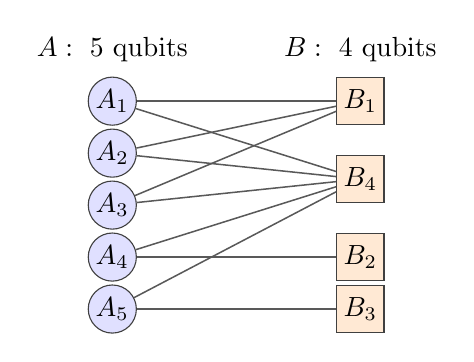
\begin{tikzpicture}[x=1.05cm,y=0.66cm,
  va/.style={circle,draw=black!75,fill=blue!12,minimum size=6mm,inner sep=1pt},
  vb/.style={rectangle,draw=black!75,fill=orange!17,minimum size=6mm,inner sep=1pt}]
\node[va] (a1) at (0,4) {$A_1$};
\node[va] (a2) at (0,3) {$A_2$};
\node[va] (a3) at (0,2) {$A_3$};
\node[va] (a4) at (0,1) {$A_4$};
\node[va] (a5) at (0,0) {$A_5$};
\node[vb] (b1) at (3,4) {$B_1$};
\node[vb] (b2) at (3,1) {$B_2$};
\node[vb] (b3) at (3,0) {$B_3$};
\node[vb] (b4) at (3,2.5) {$B_4$};
\foreach \a/\b in {a1/b1,a1/b4,a2/b1,a2/b4,a3/b1,a3/b4,a4/b2,a4/b4,a5/b3,a5/b4}
  \draw[black!65,line width=0.55pt] (\a) -- (\b);
\node at (0,5) {$A:\ 5\ \text{qubits}$};
\node at (3,5) {$B:\ 4\ \text{qubits}$};
\end{tikzpicture}

\caption{The graph of Eq.~\eqref{eq:witness}. The five circular vertices belong
to $A$ and the four square vertices to $B$. Every edge represents one ideal
controlled-$Z$ gate; every vertex receives the same phase-error probability
$q=1/200$. The diagram is drawn directly from the displayed matrix using
AI-assisted TikZ code.}
\label{fig:graph}
\end{figure}

The equations $\Gamma_3^{\mathsf T}u=0$ reduce to
$u_1+u_2+u_3=0$ and $u_4=u_5=0$. The kernel on $A$ therefore consists of
the zero vector and three weight-two vectors. The kernel on $B$ is generated
by $(1,1,1,1)$. Equation~\eqref{eq:marginal} gives
\begin{align}
 \rho_A&=\frac1{32}\bigl[I+t^2(X_1X_2+X_1X_3+X_2X_3)\bigr],\nonumber\\
 \rho_B&=\frac1{16}\bigl[I+t^4X_1X_2X_3X_4\bigr].
 \label{eq:localnine}
\end{align}
Identities on unnamed local qubits are implicit. The three pair operators on
$A$ commute, and the product of any two is the third. Setting
\begin{equation}
 a=\frac{1+3t^2}{4}=P^3+q^3,\qquad
 b=\frac{1-t^2}{4}=Pq,\qquad
 c=\frac{1-t^4}{2},
 \label{eq:abc}
\end{equation}
their four joint sectors have weights $(a,b,b,b)$. Each sector has dimension
eight, so $\rho_A$ has eigenvalue $a/8$ with multiplicity eight and $b/8$
with multiplicity twenty-four. The two sectors on $B$ have weights
$(1-c,c)$, also with dimension eight each. Hence
\begin{align}
 S_A&=3+H(a,b,b,b), & S_B&=3+h_2(c),\nonumber\\
 \Delta_3(P)&=H(a,b,b,b)-h_2(c), & S_{AB}&=9h_2(P).
 \label{eq:nineentropy}
\end{align}

At $P_0$, $t=99/100$, and the spectra are the exact rational values in
Table~\ref{tab:spectra}. Rational logarithm enclosures, described in
Appendix~\ref{app:certificate}, give
\begin{align}
 -0.004200827863112&<\Delta_3(P_0)<-0.004200827863110,\nonumber\\
 2.72683098764302&<\IA(P_0)<2.72683098764304,\nonumber\\
 2.73103181550613&<\IB(P_0)<2.73103181550615,\nonumber\\
 0.04541469233379&<h_2(P_0)<0.04541469233380.
 \label{eq:intervals}
\end{align}
The displayed decimals are deliberately wider rational bounds, not estimated
floating-point errors. In particular,
$-0.0043<\Delta_3(P_0)<-0.0042$ and $\IB>\IA>2.7$ bits.
This is a strict counterexample to Eq.~\eqref{eq:conjecture} within the
connected, rank-deficient domain, with positive coherent-information bounds
in both directions.

\begin{table}[tb]
\centering
\caption{Exact marginal spectra of the nine-qubit graph at $P_0=199/200$.
Multiplicities count separate eigenvalues. Each marginal has unit trace.}
\label{tab:spectra}
\begin{tabular}{ccc}
\toprule
Marginal & Eigenvalue & Multiplicity\\
\midrule
$\rho_A$ & $39403/320000$ & $8$\\
         & $199/320000$ & $24$\\[2pt]
$\rho_B$ & $196059601/1600000000$ & $8$\\
         & $3940399/1600000000$ & $8$\\
\bottomrule
\end{tabular}
\end{table}

\section{A family at a common noise strength}\label{sec:family}

\begin{proposition}\label{prop:family}
For every finite integer $r\geq3$, let $v_i=e_i+e_{r+1}\in\F^{r+1}$,
where $e_i$ is a standard basis vector, and let $\Gamma_r$ have rows
\begin{equation}
 v_1,\ v_1,\ v_1,\ v_2,\ldots,\ v_r.
 \label{eq:family}
\end{equation}
This matrix defines a connected simple bipartite graph with
$n_A=r+2>r+1=n_B$ and binary rank $r<n_B$. Under
Eqs.~\eqref{eq:channel}--\eqref{eq:state} at the same $P_0=199/200$,
\begin{equation}
 \Delta_r(P_0)\leq\Delta_3(P_0)<-0.0042,
 \qquad \IB(r,P_0)>\IA(r,P_0)>2.7.
 \label{eq:allr}
\end{equation}
\end{proposition}

\begin{proof}
The first $r$ columns establish independence of $v_1,\ldots,v_r$.
The last column is nonzero in every row, and every other column is nonzero,
which also proves connectivity. The local kernel on $A$ again consists of
$u_1+u_2+u_3=0$, with all other coordinates zero; the kernel on $B$ is
generated by the length-$(r+1)$ all-one vector. Thus the four $A$ sectors
still have weights $(a,b,b,b)$, and the two $B$ sectors have weights
$(1-c_r,c_r)$, where
\begin{equation}
 c_r=\frac{1-t^{r+1}}2.
 \label{eq:cr}
\end{equation}
Every sector has dimension $2^r$. The exact entropies are
\begin{align}
 S_A(r,P)&=r+H(a,b,b,b),\nonumber\\
 S_B(r,P)&=r+h_2(c_r),\nonumber\\
 S_{AB}(r,P)&=(2r+3)h_2(P).
 \label{eq:familyentropy}
\end{align}
For $1/2<P<1$, one has $0<t<1$, so $c_r$ strictly increases with $r$ and
lies in $(0,1/2)$. Since $h_2'(x)=\log_2[(1-x)/x]>0$ there,
$\Delta_r(P)\leq\Delta_3(P)$ for $r\geq3$ (strictly for $r>3$).
Equation~\eqref{eq:intervals} therefore proves the first inequality in
Eq.~\eqref{eq:allr}. Furthermore,
\begin{equation}
 \IA(r,P_0)=\IA(3,P_0)+(r-3)\bigl[1-2h_2(P_0)\bigr].
 \label{eq:slope}
\end{equation}
The bracket is positive by Eq.~\eqref{eq:intervals}, so
$\IA(r,P_0)\geq\IA(3,P_0)>2.7$. Finally,
$\IB(r,P_0)=\IA(r,P_0)-\Delta_r(P_0)>\IA(r,P_0)$.
\end{proof}

The result concerns each finite graph at a fixed physical noise parameter.
It does not require a thermodynamic limit or an extrapolation from finitely
many ranks. Each added vertex remains connected to the graph and receives
the same noise; none is a noiseless spectator.

\section{Support mechanism and physical scope}\label{sec:scope}

The role of stabilizer support can also be read from the low-noise limit.
For a fixed finite $r$ and $q\to0^+$,
$b=q+O(q^2)$, $a=1-3q+O(q^2)$, and
$c_r=(r+1)q+O_r(q^2)$. Therefore
\begin{align}
 H(a,b,b,b)&=3q\log_2(1/q)+O(q),\nonumber\\
 h_2(c_r)&=(r+1)q\log_2(1/q)+O_r(q),\nonumber\\
 \lim_{q\to0^+}\frac{\Delta_r(1-q)}{q\log_2(1/q)}&=2-r.
 \label{eq:asymptotic}
\end{align}
The constants in the $r$-dependent remainders need not be uniform in rank.
The common-$P_0$ statement of Proposition~\ref{prop:family} follows from
the exact entropies and monotonicity, not from this expansion.

Although $A$ contains $r+2$ physical qubits, its nontrivial local stabilizers
involve just the first three. In contrast, $B$'s parity stabilizer involves
all $r+1$ qubits. Independent phase noise consequently creates different
syndrome entropies on the two sides. The remaining qubits on $A$ still enter
the local dimension, the joint state, and the total entropy
$(2r+3)h_2(P)$. Omitting those factors would give the wrong coherent information.

At the pure endpoint $P=1$, both marginal entropies are $r$ and $S_{AB}=0$.
At $P=1/2$, the full state is maximally mixed, so $S_A=r+2$, $S_B=r+1$,
and $\Delta_r=1$. The interior negative difference is thus consistent with
both endpoints. No claim is made that nine qubits is the smallest possible
counterexample, that the interior sign change is unique, or that all graphs
or all noise strengths exhibit a reversal.

The operational consequence is specifically a failure of node count to select
the larger coherent-information lower bound. For the nine-qubit example,
distillation with classical communication from $A$ to $B$ has the larger
hashing lower bound, even though the receiving side is smaller. This comparison
alone does not compare optimal one-way rates, two-way distillable entanglement,
or performance of a finite-copy implementation. The model uses ideal gates,
uniform independent phase noise, no measurements or postselection, and no
perturbative truncation. Extending the result to other noise channels would
require a separate calculation.

\appendix
\section{Exact sign certificate and reproducibility}\label{app:certificate}

For each nonzero rational eigenvalue $p$, write $p=2^{-k}y$ with
$1/2\leq y\leq1$ and integer $k\geq0$, and put $z=1-y$. For any positive
integer $M$,
\begin{equation}
 L_M(y):=\sum_{j=1}^M\frac{z^j}{j}
 \ \leq\ -\ln y\ \leq\
 L_M(y)+\frac{z^{M+1}}{(M+1)(1-z)}.
 \label{eq:mercator}
\end{equation}
Indeed the omitted positive terms have denominators at least $M+1$, and
their powers sum as a geometric series. Apply the same bounds at $y=1/2$
to enclose $\ln2$. If $[l_y,u_y]$ and $[l_2,u_2]$ are these intervals, then
\begin{equation}
 k+\frac{l_y}{u_2}\ \leq\ -\log_2p\ \leq\
 k+\frac{u_y}{l_2}.
 \label{eq:surprisal}
\end{equation}
Multiplication by the nonnegative $p$ and addition with the exact
multiplicities enclose the entropy. For a difference of intervals use
$[l_x-u_y,u_x-l_y]$. With $M=96$, all arithmetic is rational;
outward rounding is used only for the displayed decimal endpoints.
This proves Eq.~\eqref{eq:intervals} without relying on a floating-point sign.

The accompanying Python script reconstructs the same spectra through the
complete phase-error ensemble of Eq.~\eqref{eq:state}. It uses the
computational-basis graph phases, takes both partial traces exactly, and
checks the full Walsh-character eigenvector equations. Thus it checks the
rational spectra without assuming the local-kernel formula. It also replays
the rank-one $K_{2,1}$ benchmark at $P=3/4$ from
Ref.~\cite[Eqs.~(25)--(27)]{Sajjad2026lowerbounds}, giving
$S_A=1+h_2(5/8)$ and $S_B=1$, and checks the seven-qubit graph of that
reference's Eq.~(28) against the kernel representation.

The supplement contains the script, expected rational spectra and entropy
enclosures, environment information, and instructions for regeneration.
It requires only the Python standard library. Finite-rank diagnostics in the
script are consistency checks; Proposition~\ref{prop:family} supplies the
argument for every finite $r\geq3$.

\section*{Statements and Declarations}
\paragraph{Data and code availability.}
All numerical inputs are explicit in the manuscript and supplementary script.
The supplement supplies exact-arithmetic reproduction code and reference
outputs. No experimental or personal data are used.

\paragraph{Use of artificial intelligence.}
OpenAI ChatGPT and Codex were used in identifying the research question,
constructing and analyzing the counterexample, developing the proof and
reproduction code, checking sources and calculations, and drafting this text
and its diagram. The writing stage used a GPT-6-based Codex assistant;
the exact model versions for all preceding stages are not established here.
AI checks are not human peer review. This local draft awaits substantive
review and approval by the named human author, including the analysis,
citations, interpretation, authorship, and applicable journal policy.

\paragraph{Funding and competing interests.}
The author's funding and competing-interest declarations remain to be supplied
and confirmed before submission.

\bibliographystyle{unsrtnat}
\bibliography{references}
\end{document}
